%\subsection{MSSM benchmark scenarios for the HL-LHC}
\subsection{Direct and indirect sensitivity to heavy Higgs bosons using MSSM benchmark scenarios}\label{Sec:9.5}
\begin{center}
\textit{by Philip Bechtle, Sven Heinemeyer, Stefan Liebler, Tim Stefaniak and Georg Weiglein}
\end{center}

%\subsubsection{Introduction}

The LHC keeps measuring the properties of the discovered Higgs boson with increasing precision. So far the measured properties are, within current experimental and theoretical uncertainties, in agreement with the SM predictions~\cite{Khachatryan:2016vau}. The MSSM~\cite{Nilles:1983ge,Haber:1984rc,Gunion:1984yn} is one of the best studied models with an extended Higgs sector. It predicts two scalar partners for all SM fermions as well as fermionic partners to all SM bosons. Contrary to the case of the SM, the MSSM contains two Higgs doublets.
This results in five physical Higgs bosons instead of the single Higgs boson in the SM. In the absence of $\mathcal{CP}$-violating phases, these are the light and heavy $\mathcal{CP}$-even Higgs bosons,  
$h$ and $H$, the $\mathcal{CP}$-odd Higgs boson, $A$, and the charged Higgs bosons, $H^\pm$.

In order to facilitate collider searches for the additional MSSM Higgs bosons, a set of new benchmark scenarios for MSSM Higgs boson searches at the LHC have been proposed recently~\cite{Bahl:2018zmf}. The scenarios are compatible -- at least over wide portions
of their parameter space -- with the most recent LHC results for the
Higgs-boson properties and the bounds on masses and couplings of new
particles. Each scenario contains one $\mathcal{CP}$-even scalar with mass around $125$\,\UGeV and SM-like couplings. However, the scenarios differ importantly in the phenomenology of the additional, so far undetected Higgs bosons.

The search for the additional Higgs bosons will continue at the LHC
Run~3 and subsequently at the HL-LHC. These benchmark scenarios, due to their distinct phenomenology of the additional Higgs bosons, serve well to assess the reach of current and future colliders. The reach can either be direct, via the search for new Higgs bosons, or indirect, via the precise measurements of the properties of the Higgs boson at $\sim 125$\,\UGeV. 

\subsubsection*{Experimental and theoretical input}

In order to analyse the potential of the HL-LHC in the exploration of the MSSM Higgs sector we evaluate the direct and indirect physics reach in two of the benchmark scenarios proposed in Ref.~\cite{Bahl:2018zmf}. The first scenario is the $M_h^{125}$: it is characterised by relatively heavy superparticles, such that the Higgs phenomenology at the LHC resembles that of a Two-Higgs-Doublet-Model with MSSM-inspired Higgs couplings. The second scenario is the $M_h^{125}(\tilde{\chi})$. It is characterised by light electroweakinos (EWinos), resulting in large decay rates of the heavy Higgs bosons $H$ and $A$ into charginos and neutralinos, thus diminishing the event yield of the $\tau^+\tau^-$~final state signatures that are used to search
for the additional Higgs bosons at the LHC. In addition, the branching ratios of the Higgs boson at $125$\,\UGeV into a pair of photons is enhanced for small values of $\tan\beta$ due to the EWinos present in the loop.

We assess the reach of direct LHC searches in the  $\tau^+\tau^-$
final state by applying the model-independent $95\%~\mathrm{CL}$
limit projections for $6~\mathrm{ab}^{-1}$ from the CMS experiment, see Sec.~\ref{sec:model_indep}, Fig.~\ref{fig:model_indep}.\footnote{We thank Martin Flechl for helpful discussions.} 
%CMS evaluated these projections both for the $m_h^{{\rm mod}+}$~scenario~\cite{Carena:2013ytb} and for 
We implemented these limits --- presented as one-dimensional (marginalised) cross section limits on either the
gluon fusion or $b\bar{b}$-associated production mode --- in the program
\texttt{HiggsBounds}~\cite{Bechtle:2008jh,Bechtle:2011sb,Bechtle:2013wla,Bechtle:2015pma} to obtain the projected $95\%~\mathrm{CL}$ exclusion in our scenarios.

We estimate the indirect reach through Higgs rate measurements by
using detailed HL-LHC signal strength projections for the individual
Higgs production times decay modes, including the corresponding
correlation matrix, as evaluated by the ATLAS and CMS experiment assuming YR18 systematic uncertainties (S2), see Sec.~\ref{sec:expcomb_prodtimesdecay}, Tab.~\ref{tab:summary_A1_5PD}.  We furthermore take cross-correlations of theoretical
rate uncertainties between future ATLAS and CMS measurements into
account. All this is done with the use of the program
\texttt{HiggsSignals}~\cite{Bechtle:2013xfa}. 
%We provide projections for both scenarios S1 and S2, where the theory uncertainties are kept at their current values, or halved, respectively.

The theory predictions are obtained from
\texttt{FeynHiggs}~\cite{Heinemeyer:1998yj,Heinemeyer:1998np,Degrassi:2002fi,Frank:2006yh,Hahn:2013ria,Bahl:2016brp,Bahl:2017aev,Bahl:2018qog},
as well as from \texttt{SusHi}~\cite{Harlander:2012pb, Harlander:2016hcx,
Harlander:2005rq,Harlander:2002wh,
Harlander:2002vv,Anastasiou:2014lda,Anastasiou:2015yha,
Anastasiou:2016cez,Degrassi:2010eu, Degrassi:2011vq,
Degrassi:2012vt,Actis:2008ug}
for gluon fusion and matched predictions for bottom-quark
annihilation~\cite{Bonvini:2015pxa,Bonvini:2016fgf,Forte:2015hba, Forte:2016sja}. We determine the theoretical uncertainties on the Higgs production cross sections as in Ref.~\cite{Bahl:2018zmf}. 
%Thus, we include renormalization- and factorization-scale uncertainties, PDF$+\alpha_s$ uncertainties as well as parametric and matching uncertainties for the $\tau^+\tau^-$~exclusion, see Ref.~\cite{Bahl:2018zmf} for details. 
For the light Higgs rate measurements we use the SM uncertainties following Ref.~\cite{deFlorian:2016spz}.

\subsubsection*{Projected HL-LHC reach}
 
Our projections in the $M_h^{125}$ and the $M_h^{125}(\tilde{\chi})$ scenario in the
($M_A, \tan\beta$) plane are presented in the left and right panel of Fig.~\ref{fig:bench}, respectively. 
%In the upper (lower) row we show the results in the S1 (S2) scenario. 
We furthermore include the current limit (magenta dotted line) for the indirect reach of the LHC in the two benchmark scenarios, as evaluated in Ref.~\cite{Bahl:2018zmf}, as well as the expected limit from current direct BSM Higgs searches by ATLAS~\cite{Aaboud:2017sjh} (red dashed line) and CMS~\cite{Sirunyan:2018zut} (green dashed line) in the $\tau^+\tau^-$ final state, using $\sim 36~\mathrm{fb}^{-1}$ of data from Run~II at $13~\mathrm{\UTeV}$.

%%%%%%%%%%%%%%%%%%% F I G U R E %%%%%%%%%%%%%%%%%%%%%%%%%%%%%%%%%%%%%%%%%%%%%%%
\begin{figure}
\begin{center}
%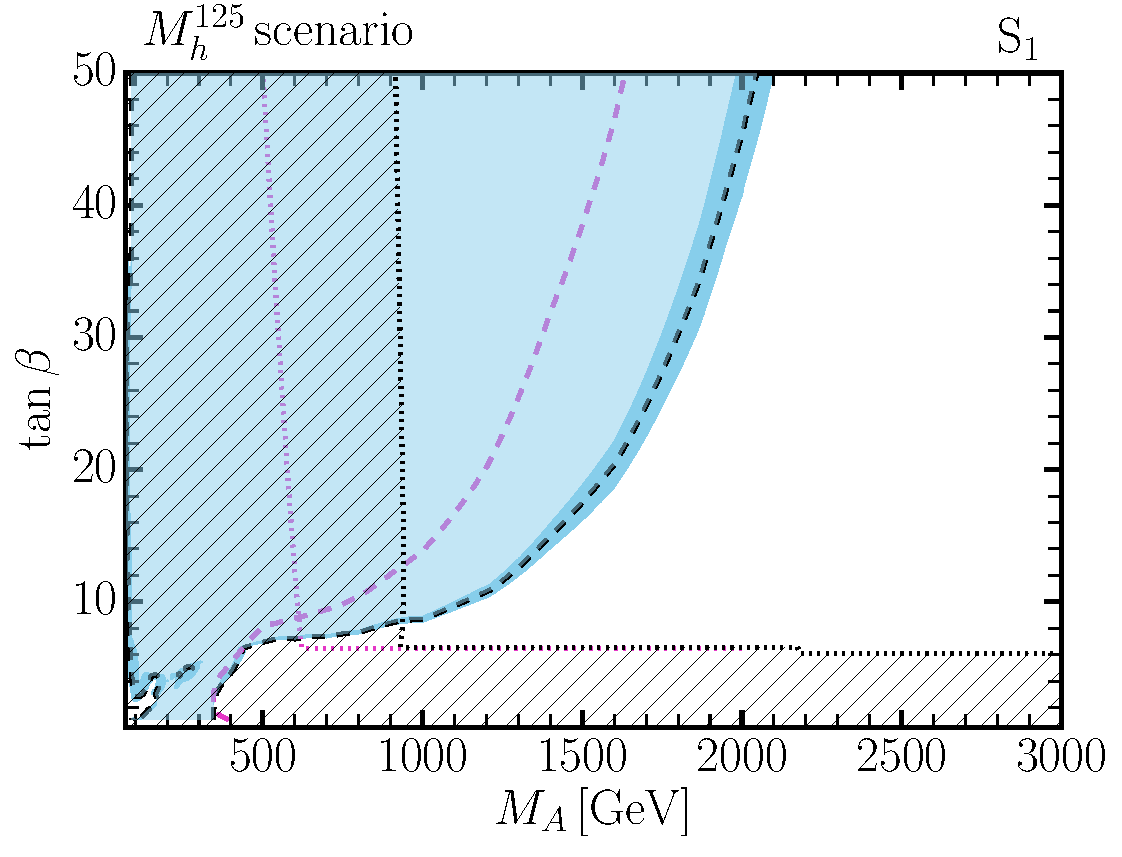
\includegraphics[width=0.5\textwidth]{\main/section9/plots/mh125S1_HBHS}\hfill
%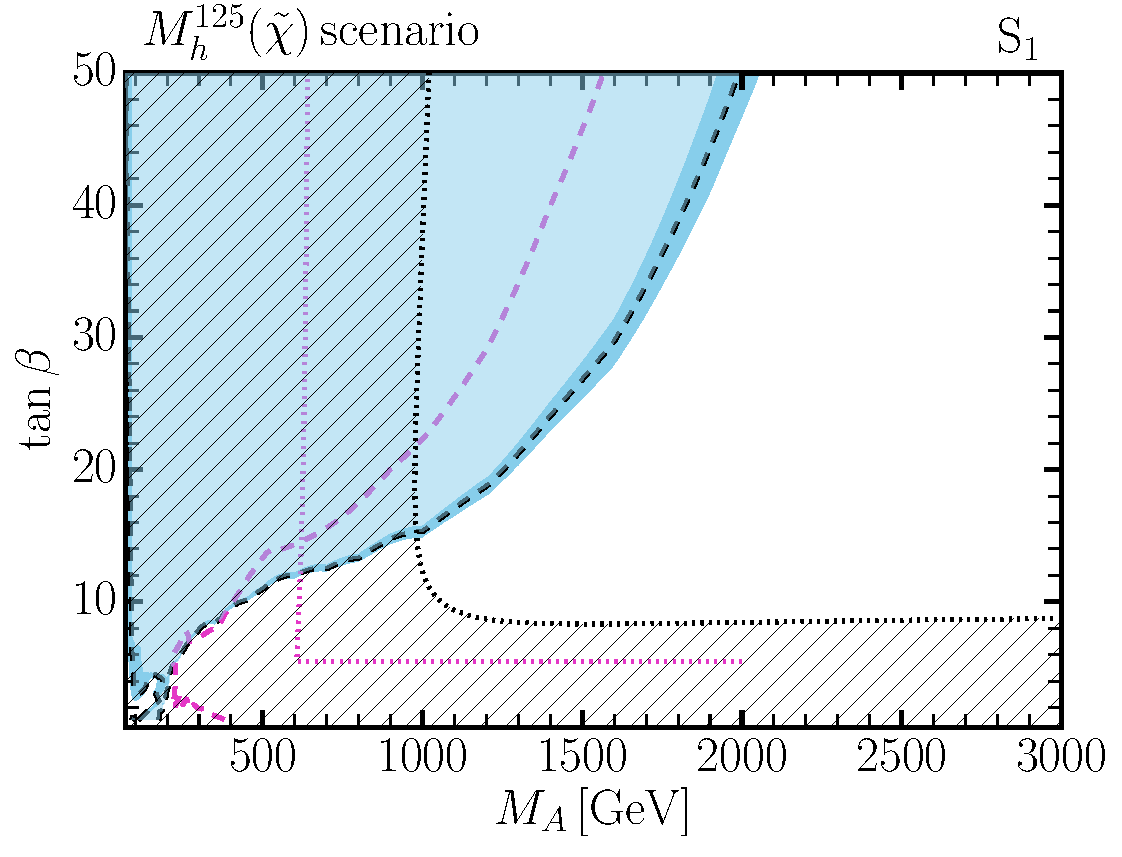
\includegraphics[width=0.5\textwidth]{\main/section9/plots/mh125-lc_S1_HBHS}\\
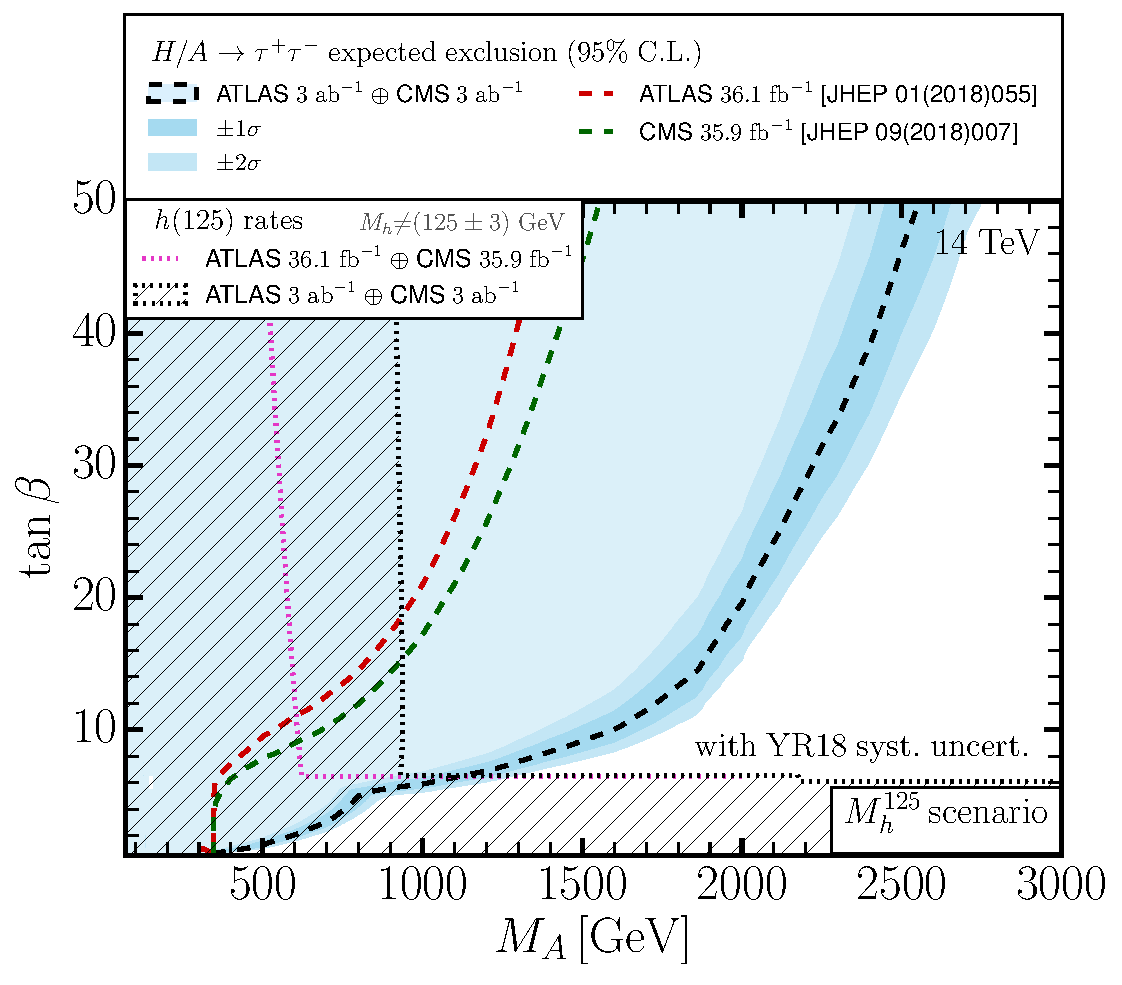
\includegraphics[width=0.5\textwidth]{\main/section9/plots/mh125S2_HBHS}\hfill
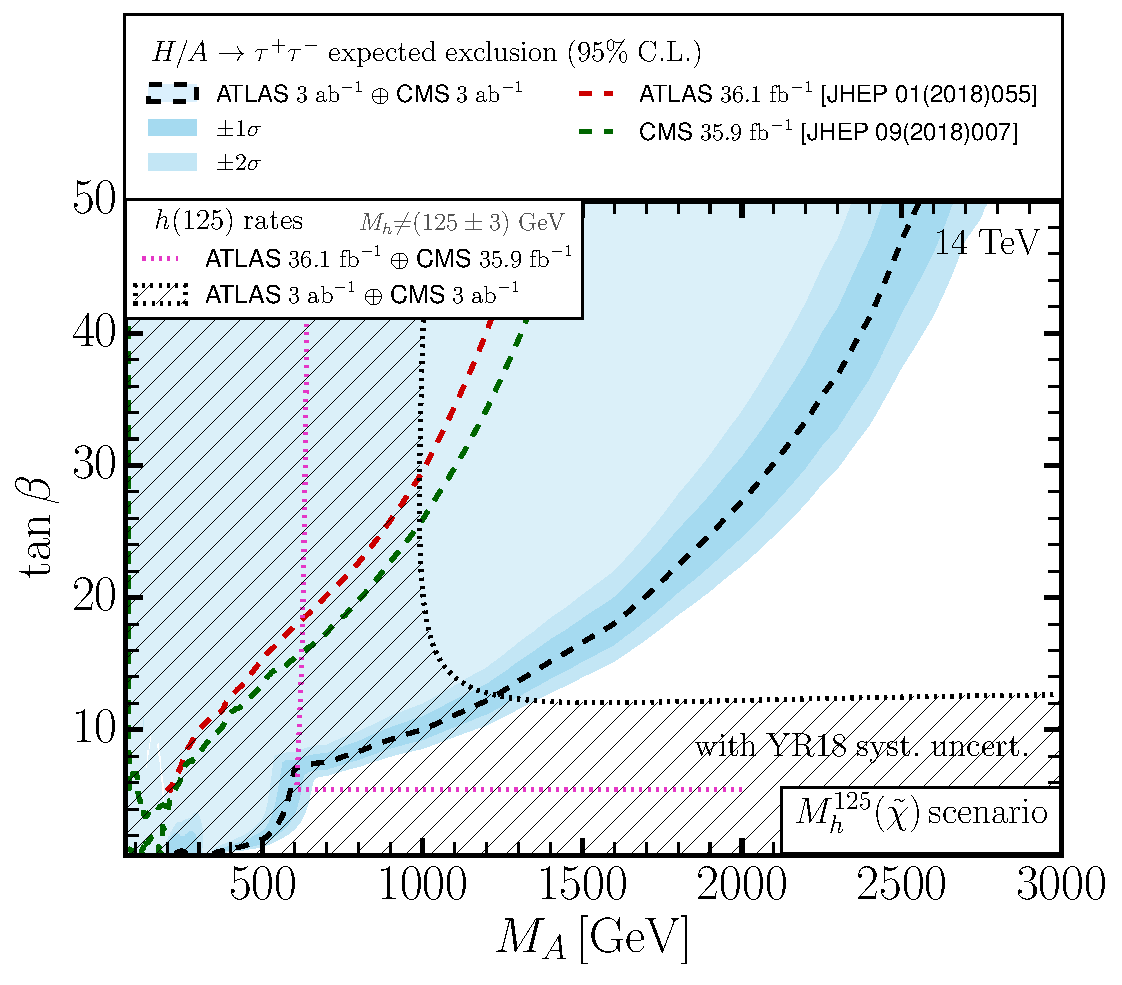
\includegraphics[width=0.5\textwidth]{\main/section9/plots/mh125-lc_S2_HBHS}
\end{center}
\caption{HL-LHC projections in the $M_h^{125}$ (\emph{left}) and
  $M_h^{125}(\tilde{\chi})$ (\emph{right}) scenario, assuming YR18 systematic uncertainties (S2). The dashed black curve and blue filled region indicate the HL-LHC reach via direct heavy Higgs searches in the $\tau^+\tau^-$ channel with $6~\mathrm{ab}^{-1}$ of data (with the dark blue regions indicating the $1$ and $2\sigma$ uncertainty), whereas 
  the red and green dashed lines show the expected limit from current searches in this channel by ATLAS~\cite{Aaboud:2017sjh} and CMS~\cite{Sirunyan:2018zut}, respectively. The current and future HL-LHC sensitivity via  combined ATLAS and CMS Higgs rate measurements is shown as magenta and black dotted contours, respectively (the latter being accompanied with a hatching of the prospectively excluded region).}
\label{fig:bench}
\end{figure}
%%%%%%%%%%%%%%%%%%% F I G U R E %%%%%%%%%%%%%%%%%%%%%%%%%%%%%%%%%%%%%%%%%%%%%%%

Within the $M_h^{125}$ scenario the reach via measurements of the Higgs signal strengths extends to $M_A$ values of around $900$\,\UGeV. The horizontal contour excluding $\tan\beta$ values less than 6 is due to the light Higgs mass being below $122$\,\UGeV, where the interpretation of the observed Higgs signal in terms of the light $\mathcal{CP}$-even MSSM Higgs boson $h$ becomes invalid. The direct heavy Higgs searches in the $\tau^+\tau^-$ final state will probe the parameter space up to $M_A \le 2550$\,\UGeV for $\tan\beta = 50$, and up to $M_A \le 2000$\,\UGeV at $\tan\beta = 20$. 

The picture is somewhat different in the $M_h^{125}(\tilde{\chi})$ scenario. Here the large branching ratio of the heavy neutral Higgs boson decaying to charginos and neutralinos leads to a strongly reduced direct reach of heavy Higgs to $\tau^+\tau^-$ searches. While at large values of $\tan\beta \sim 50$  the reach is only slightly weaker than in the $M_h^{125}$ scenario, at $\tan\beta = 20$ it is significantly reduced to $M_A \le 1700$\,\UGeV. In order to overcome this, dedicated searches for the decays of $H$ and $A$ to charginos and neutralinos will have to be devised. On the other hand, Higgs rate measurements are an important complementary probe. They exclude
$M_A \le 950$\,\UGeV and $\tan\beta \le 12.5$. While the bound in $M_A$
is induced through Higgs coupling modifications arising from
non-decoupling, values of $\tan\beta\le 12.5$ feature a too-large enhancement of the $h\to \gamma\gamma$ partial width. The combination of direct and indirect bounds yields
a lower limit of $M_A \ge 1250$\,\UGeV in the $M_h^{125}(\tilde{\chi})$ scenario.

In summary, the HL-LHC has the potential, using the combined direct and indirect reach, to probe the MSSM Higgs sector up to $M_A \sim 900$-$1000$\,\UGeV and possibly beyond, depending on the details of the MSSM scenario. Values larger than that, as predicted, e.g., by GUT based models~\cite{Buchmueller:2013rsa,Buchmueller:2014yva,Bechtle:2015nua,Bagnaschi:2016afc,Bagnaschi:2016xfg,Costa:2017gup} or Finite Unified Theories~\cite{Heinemeyer:2013nza,Heinemeyer:2018roq,Heinemeyer:2018zpw}, or allowed by global fits of the phenomenological MSSM~\cite{Bechtle:2016kui,Bagnaschi:2017tru} would remain uncovered. To explore these regions an energy upgrade and/or refined Higgs signal strength measurements (e.g.\ at an $e^+e^-$ collider~\cite{Moortgat-Picka:2015yla}) will be
necessary.